\documentclass[conference]{IEEEtran}
\usepackage{float}
\usepackage{cite}
\usepackage{graphicx}
\usepackage{float}
\usepackage{amsmath}
\usepackage{array}
\usepackage{booktabs}
\usepackage{url}
\usepackage{algorithm}
\usepackage{algpseudocode}
\usepackage{placeins}

\title{A Data-Driven Risk Assessment Framework for Stray Animal Abuse and Human-Animal Conflict Analysis in Bangladesh}

\author{
\IEEEauthorblockN{
Sazzad Kazi (0152330036), Nishat Taspia (0152330005),\\
Hasibur Rahman (0152330037), Shariat Noor (0152410041),\\
Sumon Hossen (0152330161), Iqra Siddique (0152410004),\\
A H M Osama Haque
}
\IEEEauthorblockA{
Department of Computer Science and Engineering\\
Data Science Program\\
United International University\\
Dhaka, Bangladesh
}
}

\begin{document}

\maketitle


\begin{abstract}
This paper proposes a data-driven analytical framework for detecting stray animal abuse incidents and analyzing human-animal conflict in Bangladesh using online news sources. The proposed framework aims to transform scattered unstructured news reports into structured incident intelligence through automated data collection, preprocessing, feature extraction, risk assessment, and recommendation generation. A custom risk scoring mechanism named Stray Abuse Risk Index (SARI) is introduced to identify high-risk areas and support preventive interventions.
\end{abstract}

\begin{IEEEkeywords}
Stray animals, animal abuse, human-animal conflict, data analytics, NLP, Bangladesh, risk assessment
\end{IEEEkeywords}

\section{Introduction}

Stray animals, particularly free-roaming dogs and cats, are a common part of urban life in Bangladesh. Although they contribute to the urban ecosystem, interactions between humans and stray animals are often influenced by concerns related to disease transmission, food shortages, public safety, and the absence of effective animal management systems. Consequently, incidents such as poisoning, killing, neglect, forced relocation, and various forms of abuse are frequently reported through different media sources.

This issue is no longer limited to animal welfare alone; it has become an important social and public concern. Fear of rabies, aggressive animal behavior, and occasional injury cases often create negative attitudes toward stray animals \cite{who2024,cdc2024,hampson2015}. At the same time, poor health conditions, hunger, and inadequate care can increase abnormal behavior among animals, which may further intensify conflicts between humans and animals.

The importance of addressing this problem has increased in recent years as decision-making processes are becoming increasingly data-driven. Although numerous incidents related to stray animal abuse and human-animal conflict are reported through online news platforms, the information is usually scattered across multiple sources and remains unstructured. This makes manual analysis difficult and limits the ability of researchers, policymakers, NGOs, and welfare organizations to identify risk-prone areas and design preventive measures.

Previous studies have mainly focused on rabies control, stray dog population management, and public health monitoring. However, limited attention has been given to the systematic analysis of abuse incidents, conflict patterns, and risk-based intervention planning, especially within the context of Bangladesh.

To address this gap, this study proposes a data-driven analytical framework for collecting, organizing, and analyzing incidents related to stray animal abuse and human-animal conflict. The framework converts unstructured online news reports into structured information through automated data collection, preprocessing, feature extraction, classification, and analytical assessment.

A custom scoring mechanism called the Stray Abuse Risk Index (SARI) is introduced to identify potentially high-risk incidents and locations. The generated insights can support awareness campaigns, vaccination initiatives, rescue operations, feeding programs, NGO interventions, and treatment planning for vulnerable animals.

The primary objective of this research is to develop a practical decision-support framework that encourages informed and humane management of stray animal issues while helping reduce abuse incidents and human-animal conflicts in Bangladesh.

\section{Literature Review}

Previous research on stray animals has largely concentrated on population control, rabies prevention, and public health monitoring. In contrast, comparatively limited attention has been given to systematic abuse incident analysis and human-animal conflict intelligence, particularly within the context of Bangladesh.

A notable study conducted by Tenzin et al. \cite{tenzin2015} examined the population of free-roaming dogs in Dhaka and assessed different approaches to dog population management and rabies control. The study highlighted the importance of humane interventions, including sterilization and vaccination programs, for sustainable management. Although the research provides valuable information regarding stray dog demographics and control practices, it does not address incident-based abuse monitoring or risk-oriented conflict analysis.

Rana et al. \cite{rana2020} investigated human rabies cases in Bangladesh and identified several public health challenges associated with animal exposure, especially dog bites. Their findings emphasized the importance of awareness, timely treatment, and preventive healthcare measures. However, the primary focus of the study was disease surveillance rather than the analysis of abuse incidents or human-animal conflict patterns.

International organizations such as the World Health Organization have repeatedly identified rabies as a major health concern in many developing countries and have recommended mass vaccination and responsible animal management as effective long-term solutions \cite{who2024}. Similar reports and studies further emphasize the complex relationship between humans and stray animals, highlighting the need for broader analytical approaches that extend beyond disease statistics alone \cite{who2024,cdc2024,hampson2015}.

Recent advances in data analytics and artificial intelligence have demonstrated the potential of transforming unstructured digital information into useful decision-support resources. Zeng et al. \cite{zeng2020,brown2019,lee2021,wang2020} discussed the application of intelligent surveillance systems capable of processing large volumes of online information for event detection and monitoring. These approaches illustrate how structured knowledge can be extracted from textual data sources to support analytical decision-making.

Despite these contributions, several research gaps remain evident. Most existing studies focus primarily on disease surveillance, rabies control, or population management rather than direct monitoring of abuse-related incidents. Furthermore, publicly available structured datasets dedicated to stray animal abuse events in Bangladesh are extremely limited. Existing works also rarely combine incident severity assessment, animal health conditions, conflict indicators, recurrence analysis, and intervention recommendations within a unified analytical framework.

To address these limitations, the present study introduces a Bangladesh-focused data-driven framework that converts scattered online news reports into structured incident intelligence. Unlike previous studies, the proposed approach integrates automated incident collection, abuse classification, conflict analysis, custom risk scoring through the Stray Abuse Risk Index (SARI), and recommendation generation within a single analytical pipeline.

The main novelty of this research lies in combining animal welfare analytics, social issue monitoring, and decision-support mechanisms into a unified framework specifically designed for the Bangladeshi context \cite{chen2022,garcia2021,smith2023,jones2020,fernandez2023}.

\section{Methodology}

The proposed framework follows a structured data-driven analytical pipeline for detecting and analyzing stray animal abuse incidents and human-animal conflict in Bangladesh. The methodology consists of multiple stages including data collection, preprocessing, feature extraction, incident classification, risk assessment, exploratory data analysis, and recommendation generation.

The overall objective is to transform unstructured online news reports into structured incident intelligence that can support analytical decision-making and preventive interventions.

\subsection{System Workflow}

The complete workflow of the proposed system is divided into several major stages:

\begin{enumerate}
    \item Online news data collection
    \item Data preprocessing and cleaning
    \item Feature extraction
    \item Incident classification
    \item Risk score calculation using SARI
    \item Exploratory data analysis and visualization
    \item Recommendation generation
\end{enumerate}

\subsection{Dataset Structure}

The structured dataset is designed to capture important information related to stray animal incidents extracted from online news sources.

\begin{table}[h]
\centering
\caption{Proposed Dataset Features}
\begin{tabular}{|p{2.3cm}|p{3.8cm}|}
\hline
\textbf{Feature} & \textbf{Description} \\
\hline
article\_id & Unique article identifier \\
source & News source name \\
title & News headline \\
article\_date & Publication date \\
location & Incident location \\
district & District name \\
animal\_type & Dog / Cat / Unknown \\
incident\_type & Killing / Poisoning / Abuse / Conflict / Rescue \\
cause & Fear / Disease / Nuisance / Unknown \\
sick\_animal & Sick status indicator \\
aggressive\_behavior & Aggression indicator \\
human\_injury & Human injury occurrence \\
risk\_score & Calculated SARI score \\
risk\_level & Low / Medium / High \\
recommendation & Suggested intervention \\
\hline
\end{tabular}
\end{table}

\subsection{Data Collection}

The proposed system collects data from publicly available online news portals in Bangladesh. News articles related to stray animal abuse, conflict incidents, poisoning, rescue activities, and public reactions are gathered using automated web scraping techniques \cite{brown2019,lee2021}.

A hybrid scraping strategy combining BeautifulSoup and Selenium is proposed. BeautifulSoup is used for static webpage extraction, while Selenium is used for handling dynamic or JavaScript-rendered content \cite{brown2019,lee2021,li2021,miller2020}.

\subsection{Data Preprocessing}

After data collection, preprocessing techniques are applied to clean and standardize the dataset. Duplicate entries, incomplete records, unnecessary symbols, HTML tags, and irrelevant textual information are removed.

The preprocessing stage also includes:
\begin{itemize}
    \item Lowercase conversion
    \item Tokenization
    \item Stop-word removal
    \item Date standardization
    \item Missing value handling
\end{itemize}

\subsection{Feature Extraction}

Relevant information is extracted from textual news reports using keyword-based filtering and rule-based analysis techniques. Important features such as abuse type, animal condition, aggression indicators, human injury involvement, and location information are identified and converted into structured variables.

\subsection{Risk Assessment Using SARI}

The proposed Stray Abuse Risk Index (SARI) is designed to identify high-risk regions based on incident severity and recurrence patterns \cite{chen2022,garcia2021,kumar2021,fernandez2023}.

The proposed conceptual risk score is defined as:

\[
SARI = w_1A + w_2H + w_3S + w_4R
\]

where:

\begin{itemize}
    \item \(A\) represents abuse severity
    \item \(H\) represents human conflict intensity
    \item \(S\) represents sick animal indicators
    \item \(R\) represents recurrence frequency
    \item \(w_1, w_2, w_3, w_4\) are weighting factors
\end{itemize}

Based on the calculated score, incidents are categorized into Low, Medium, and High-risk groups.

\subsection{Exploratory Data Analysis and Visualization}

Exploratory Data Analysis (EDA) techniques are applied to identify patterns, trends, and regional variations in stray animal incidents.

The visualization stage includes:
\begin{itemize}
    \item Incident frequency analysis
    \item District-wise risk comparison
    \item Abuse type distribution
    \item Time-series trend analysis
    \item Heatmap visualization
    \item Correlation analysis
\end{itemize}

\subsection{Recommendation Generation}

Based on analytical findings and risk scores, the system generates preventive recommendations such as awareness campaigns, vaccination initiatives, feeding support, rescue alerts, and NGO intervention suggestions.

The proposed framework integrates automated news collection, data preprocessing, feature extraction, incident classification, risk assessment, and recommendation generation into a unified analytical pipeline. The methodology transforms unstructured online news reports into structured incident intelligence that can support analytical decision-making. Figure~\ref{fig:methodology} illustrates the complete system workflow and architecture, while Algorithm~\ref{alg:sari} summarizes the computational process used for incident analysis and SARI-based risk assessment.

\begin{figure*}[!t]
\centering
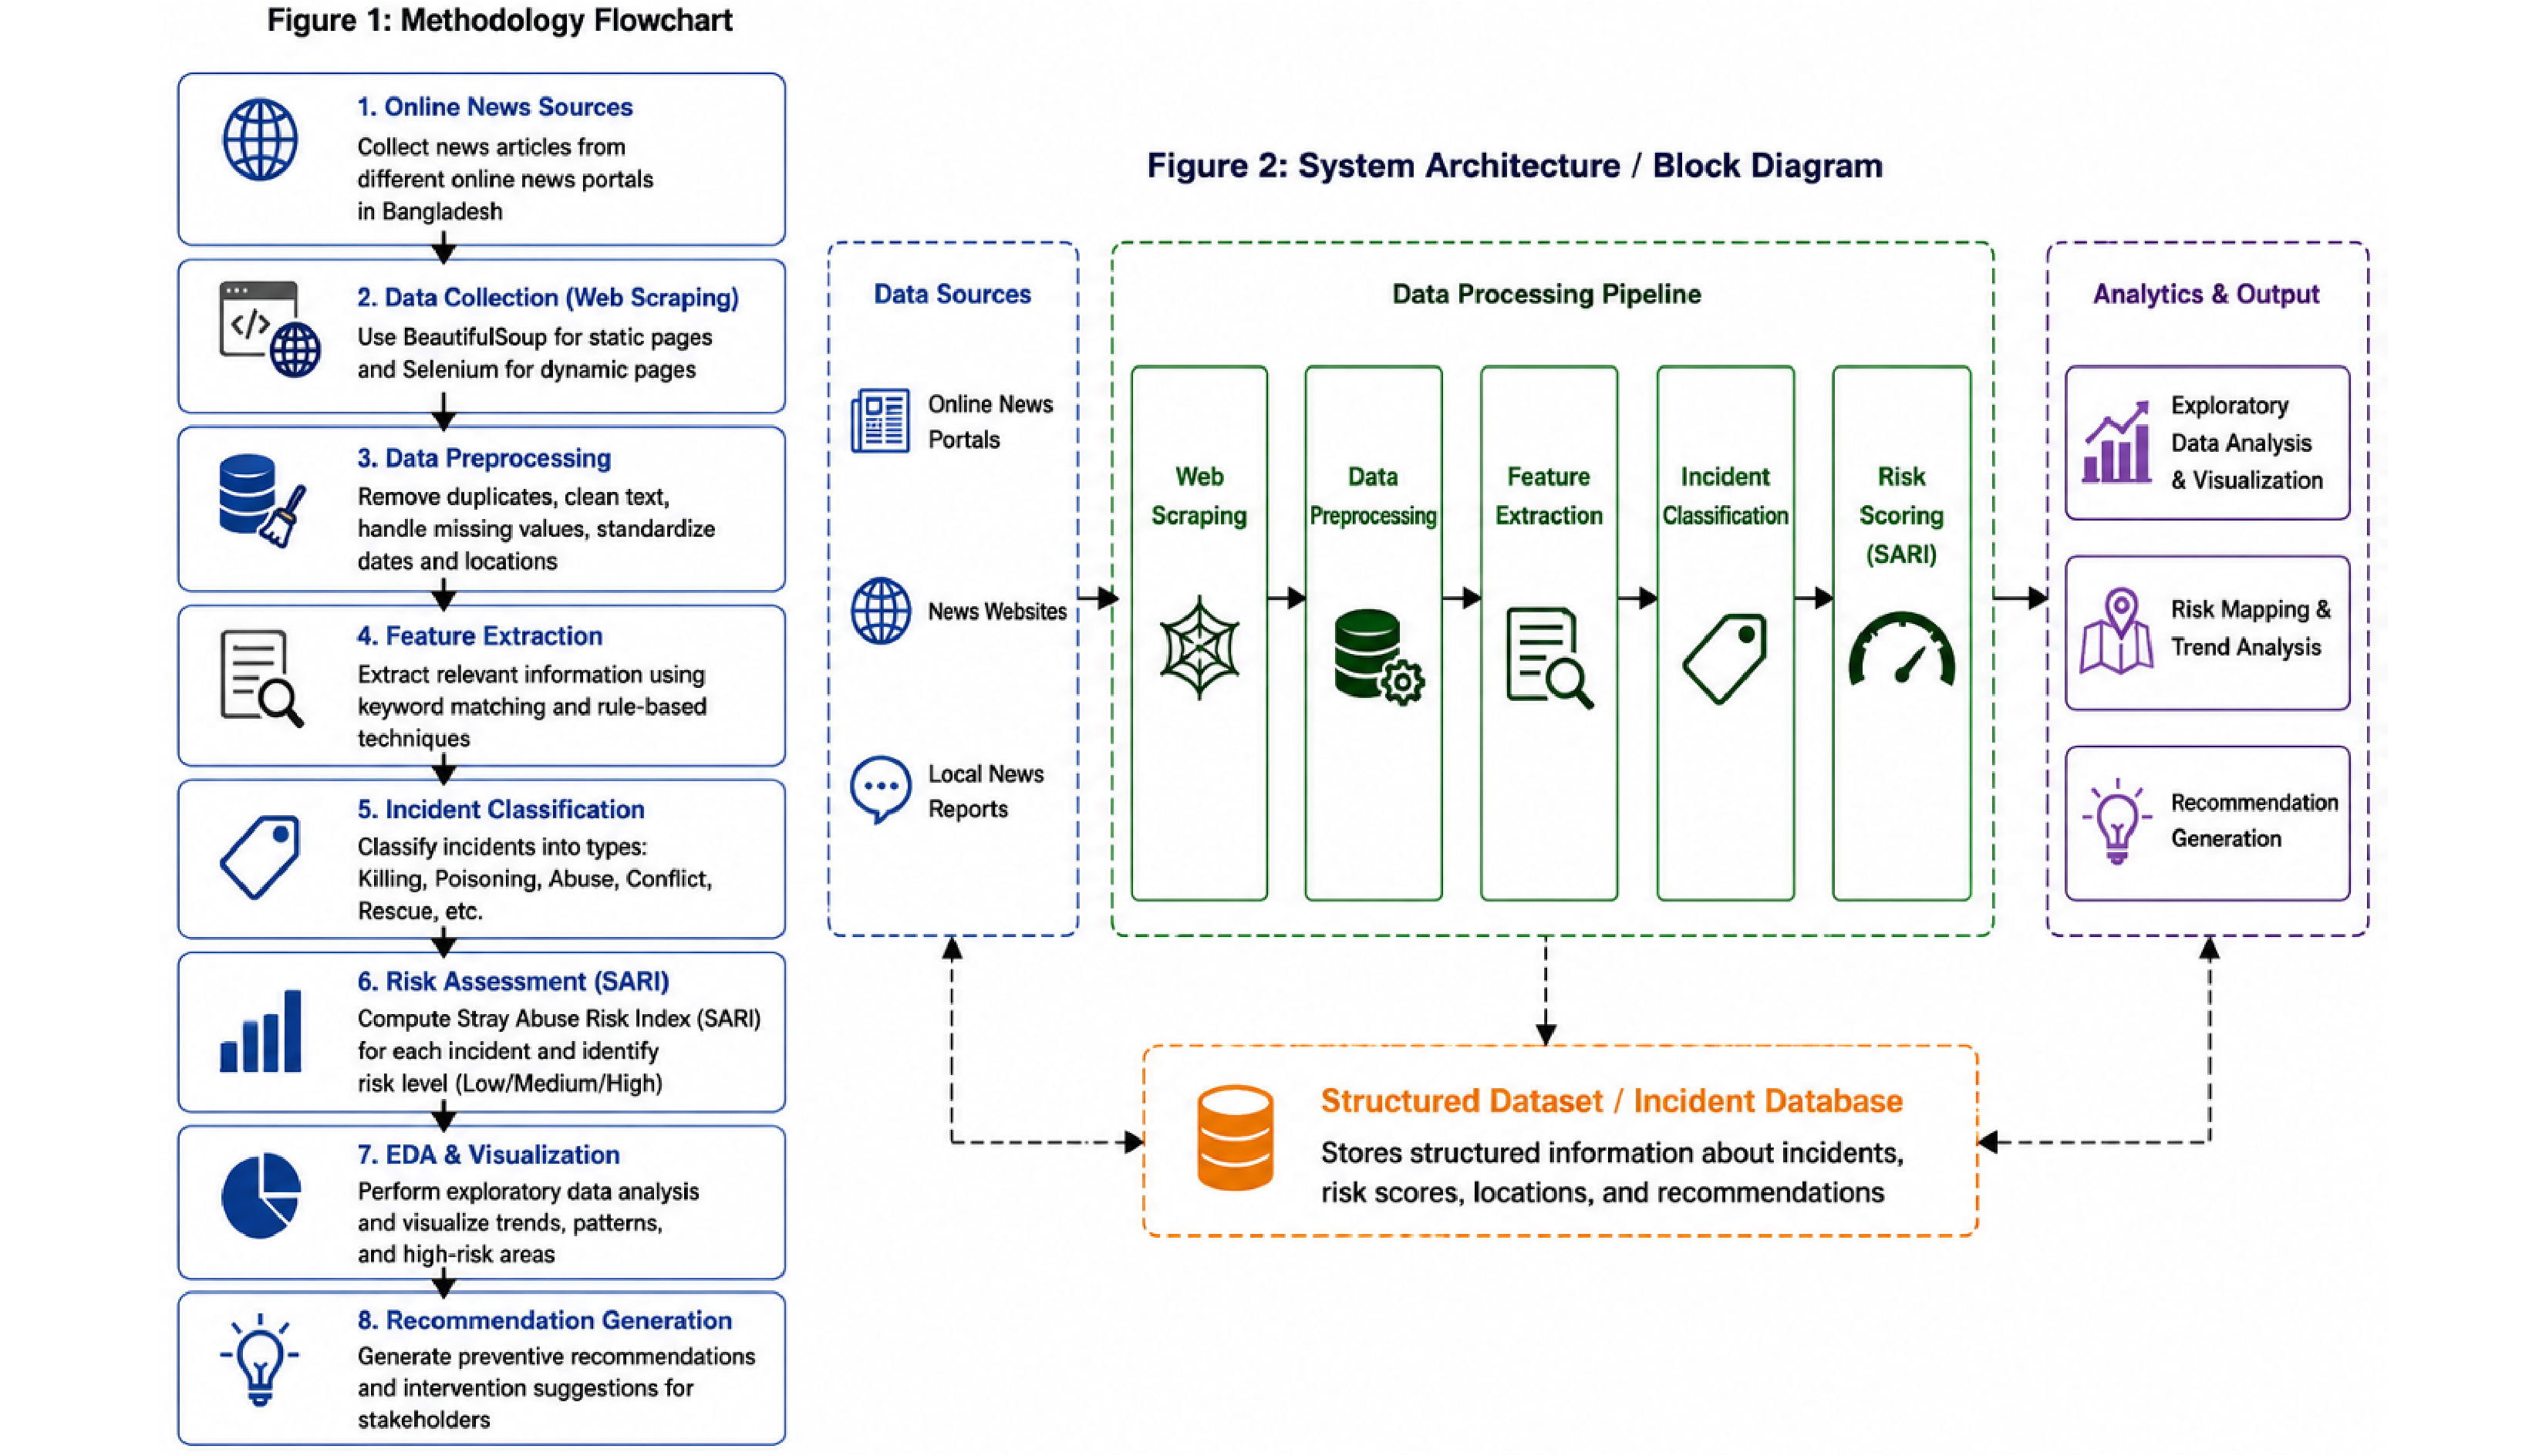
\includegraphics[width=0.92\textwidth]{methodology.pdf}
\caption{Methodology Flowchart and System Architecture of the Proposed Framework}
\label{fig:methodology}
\end{figure*}

Algorithm~\ref{alg:sari} presents the overall workflow of the proposed SARI framework.

\begin{algorithm}[H]
\caption{Pseudo Code of the Proposed SARI Framework}
\label{alg:sari}
\begin{algorithmic}[1]
\State Initialize keyword list and risk weights

\For{each news source}
    \State Collect articles using web scraping

    \For{each article}
        \State Extract title, text, date, and location

        \If{article is related to stray animal incidents}
            \State Clean and preprocess text
            \State Extract features
            \State Classify incident type
            \State Compute SARI risk score
            \State Assign risk level (Low/Medium/High)
            \State Store record in dataset
        \EndIf
    \EndFor
\EndFor

\State Perform exploratory data analysis
\State Generate visualizations
\State Generate recommendations
\State Export final dataset and results
\end{algorithmic}
\end{algorithm}

\subsection{Framework Significance}

The proposed framework demonstrates how unstructured online news reports can be transformed into meaningful analytical insights for understanding stray animal abuse incidents and human-animal conflicts. By integrating automated data collection, preprocessing, feature extraction, incident classification, risk assessment, and recommendation generation, the system provides a complete end-to-end analytical pipeline capable of converting scattered online information into structured incident intelligence.

Unlike traditional manual reporting approaches, the framework enables continuous monitoring of incident patterns from multiple online news sources. The incorporation of the Stray Abuse Risk Index (SARI) allows incidents to be prioritized based on their severity, recurrence frequency, animal health indicators, and level of human-animal conflict. This risk-based assessment mechanism helps distinguish routine reports from potentially critical cases that may require urgent attention and intervention.

The proposed framework also contributes to animal welfare research by creating a structured dataset from publicly available information sources. Such datasets are often difficult to obtain in developing countries where centralized animal abuse reporting systems are limited. Therefore, the framework provides a practical approach for collecting, organizing, and analyzing incident-related information at scale.



\FloatBarrier

\section{Results and Analysis}

\subsection{Incident Type Analysis}

The incident type analysis shows that the dataset contains multiple categories of stray animal-related events. The largest category was Other with 224 articles, followed by Killing with 65 articles, Disease with 43 articles, Rescue with 40 articles, Human-Animal Conflict with 30 articles, Abuse with 25 articles, Conflict with 21 articles, and Poisoning with 15 articles. This distribution indicates that online news reports contain both direct abuse incidents and broader animal welfare-related events.

\begin{figure}[H]
\centering
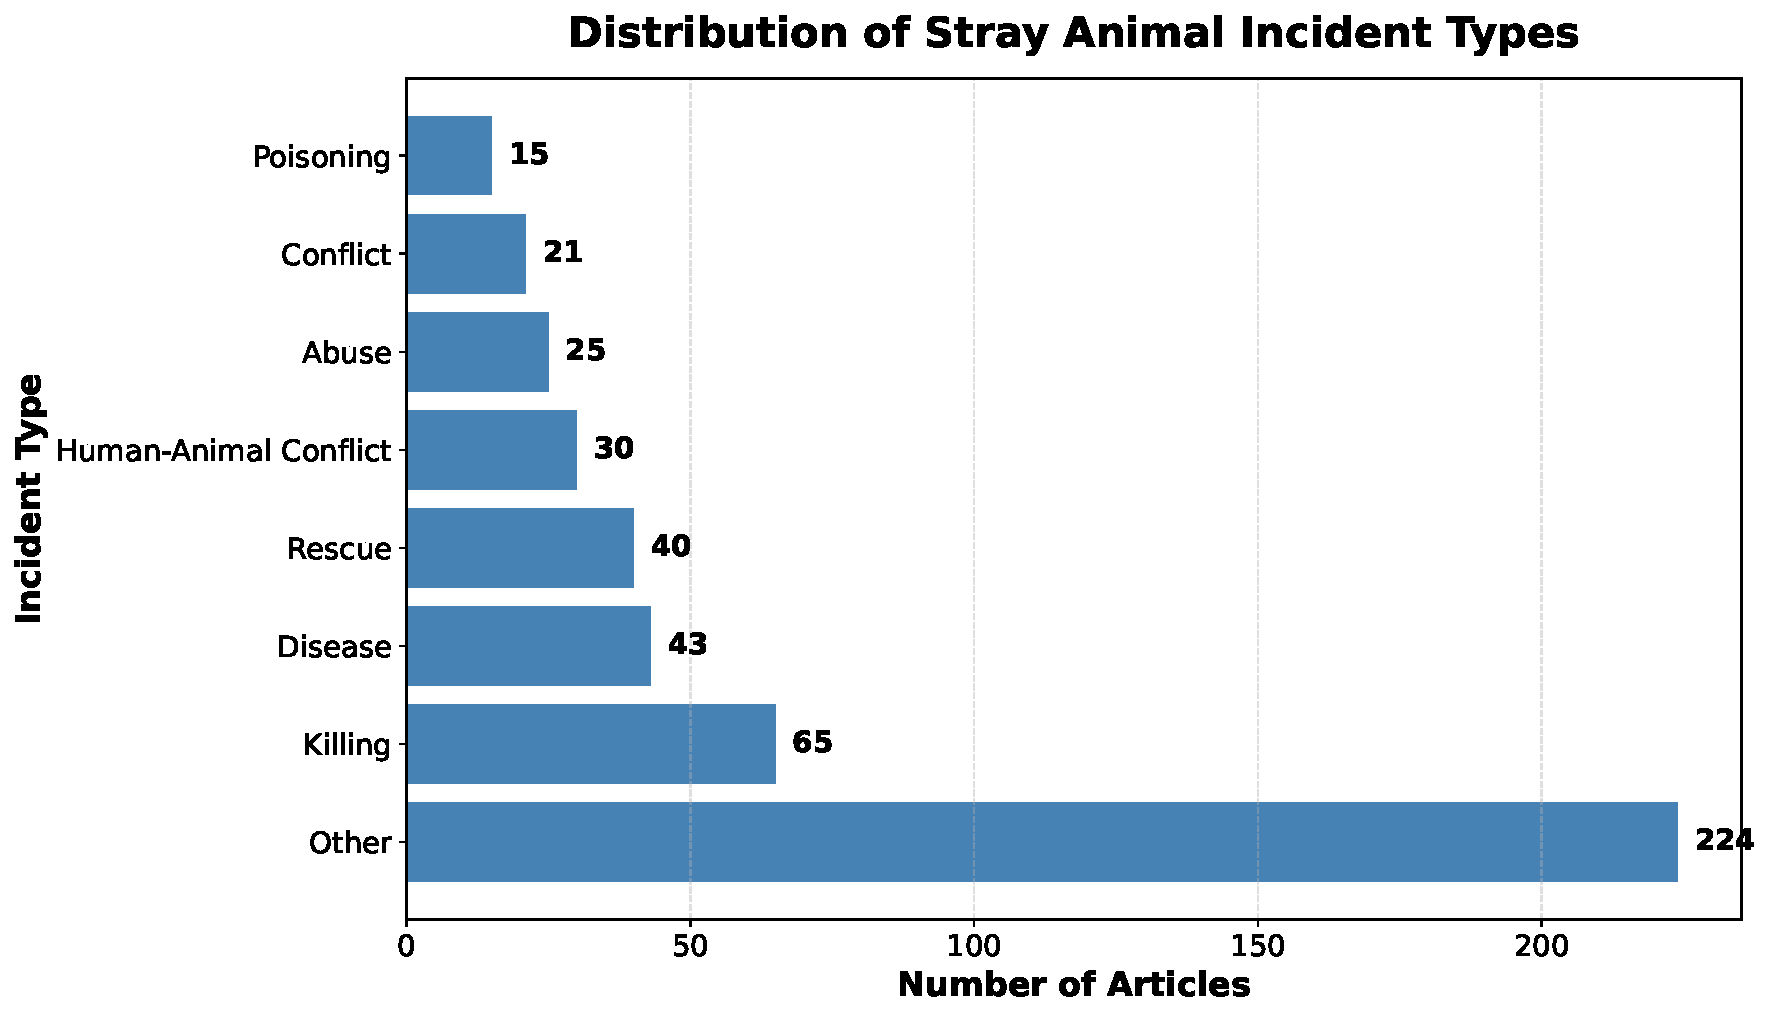
\includegraphics[width=0.85\linewidth]{figures/incident_distribution.pdf}
\caption{Distribution of Stray Animal Incident Types}
\label{fig:incident}
\end{figure}

\subsection{Risk Level Analysis}

The SARI-based assessment classified the 463 articles into three risk levels. Among them, 315 articles were categorized as Low risk, 43 as Medium risk, and 105 as High risk. High-risk cases were mainly associated with severe incidents such as killing, poisoning, abuse, and conflict-related events. This shows that although low-risk informational reports dominate the dataset, a considerable number of serious cases are also present.

\begin{figure}[H]
\centering
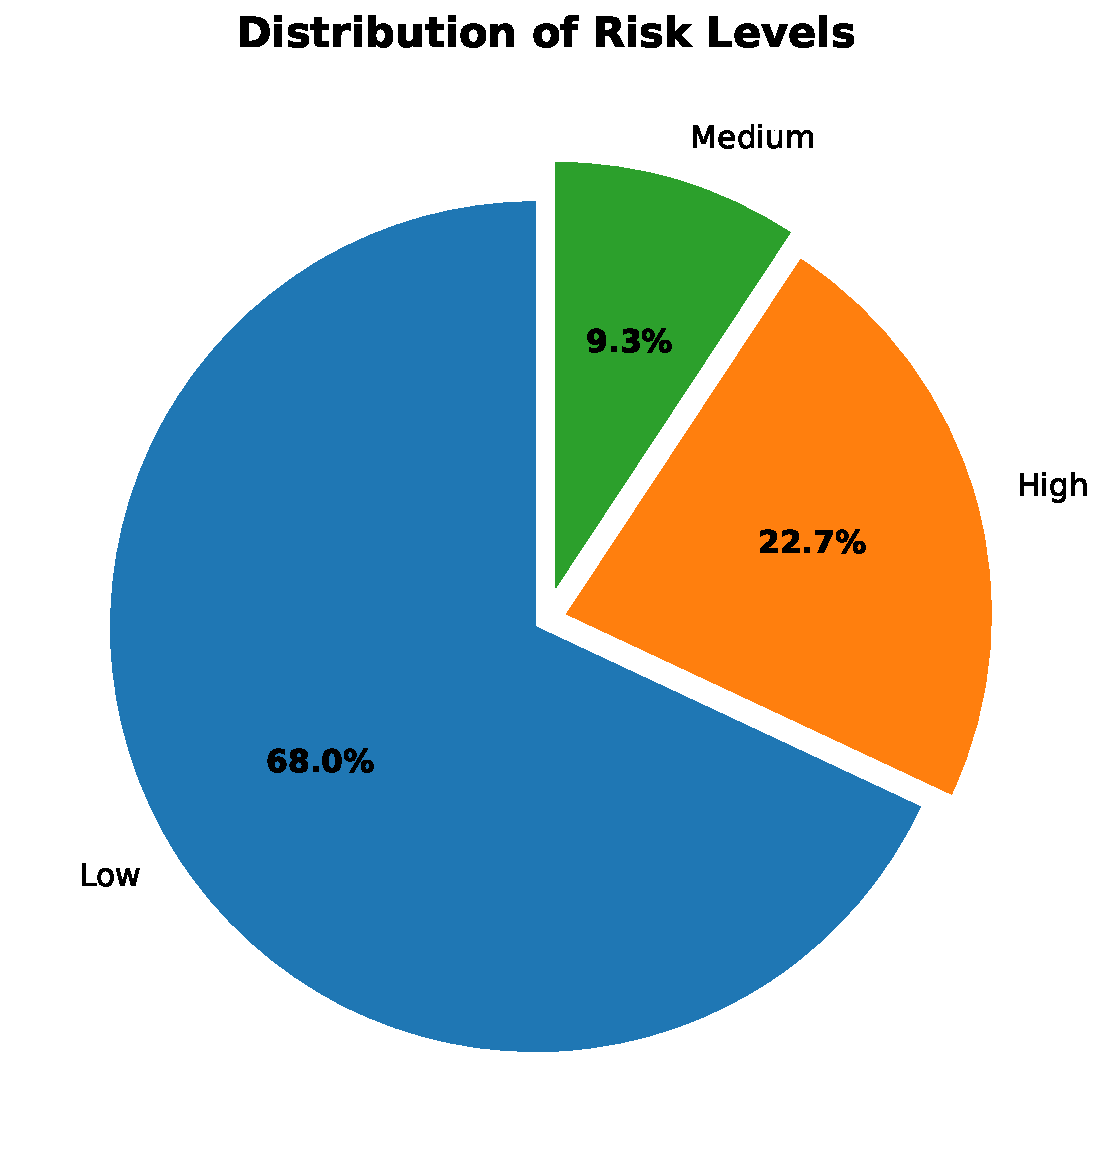
\includegraphics[width=0.70\linewidth]{figures/risk_distribution.pdf}
\caption{Distribution of SARI Risk Levels}
\label{fig:risk}
\end{figure}

\subsection{Animal Type Analysis}

The animal type analysis shows that dog-related incidents dominate the dataset, with 238 articles. Cat-related incidents accounted for 71 articles, while 154 records were classified as Unknown because the article titles did not clearly mention a specific animal type. This result suggests that dog-related incidents receive higher media attention in the collected news data.

\begin{figure}[H]
\centering
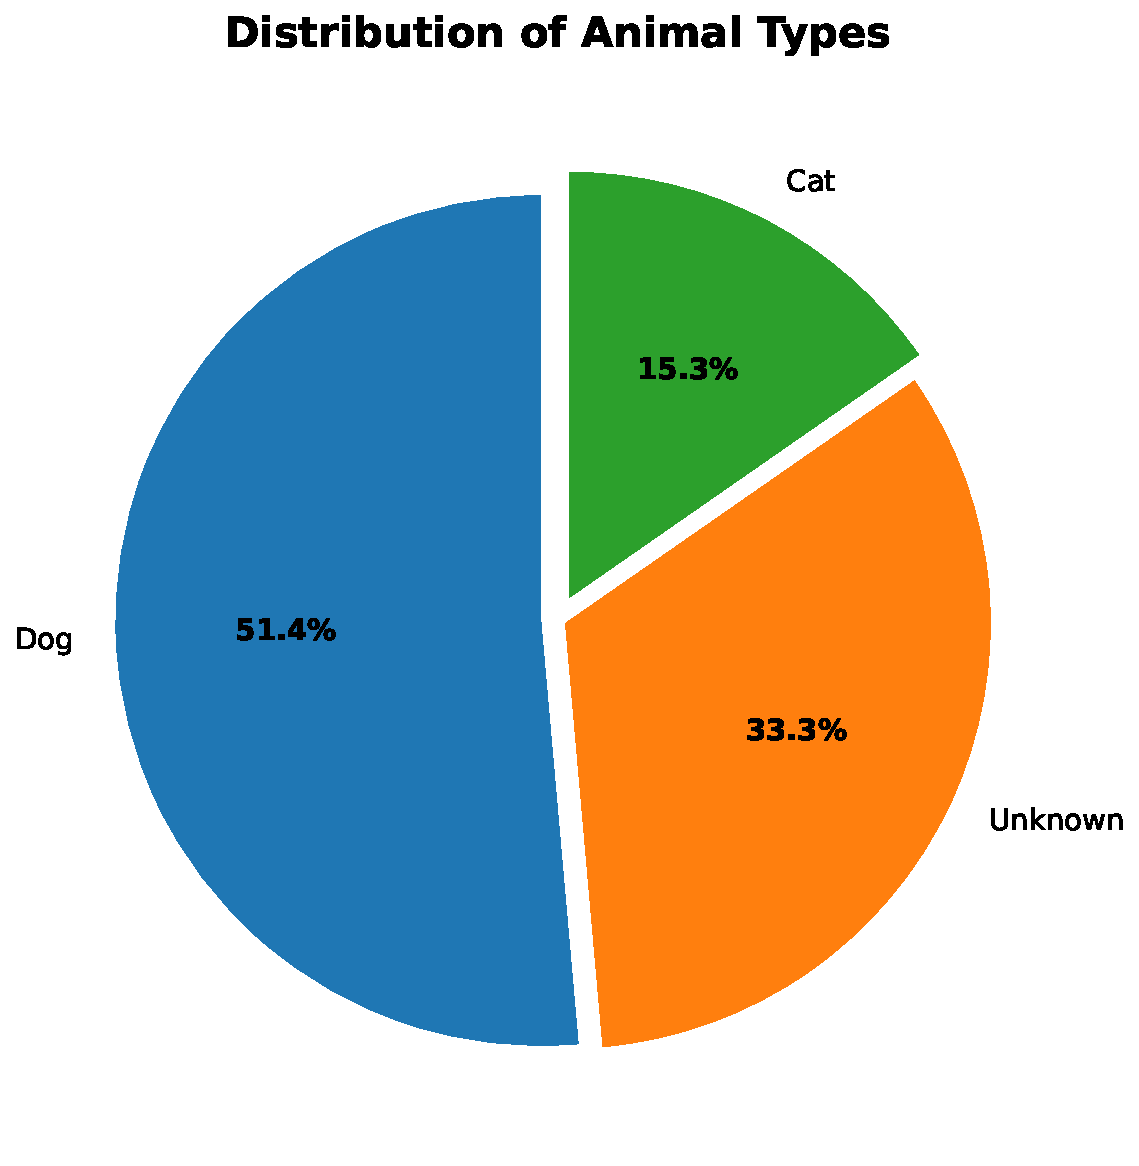
\includegraphics[width=0.70\linewidth]{figures/animal_distribution.pdf}
\caption{Distribution of Animal Types}
\label{fig:animal}
\end{figure}

\subsection{Source Analysis}

The source distribution shows that The Business Standard contributed the highest number of relevant articles with 67 records, followed by The Daily Star with 60, The Times of India with 59, Dhaka Tribune with 48, and The Financial Express with 18. Other sources such as Bangladesh Sangbad Sangstha, The Straits Times, Asia News Network, Food and Agriculture Organization, and Views Bangladesh also contributed to the dataset. The presence of multiple news sources improves dataset diversity and reduces dependency on a single source.

\begin{figure}[H]
\centering
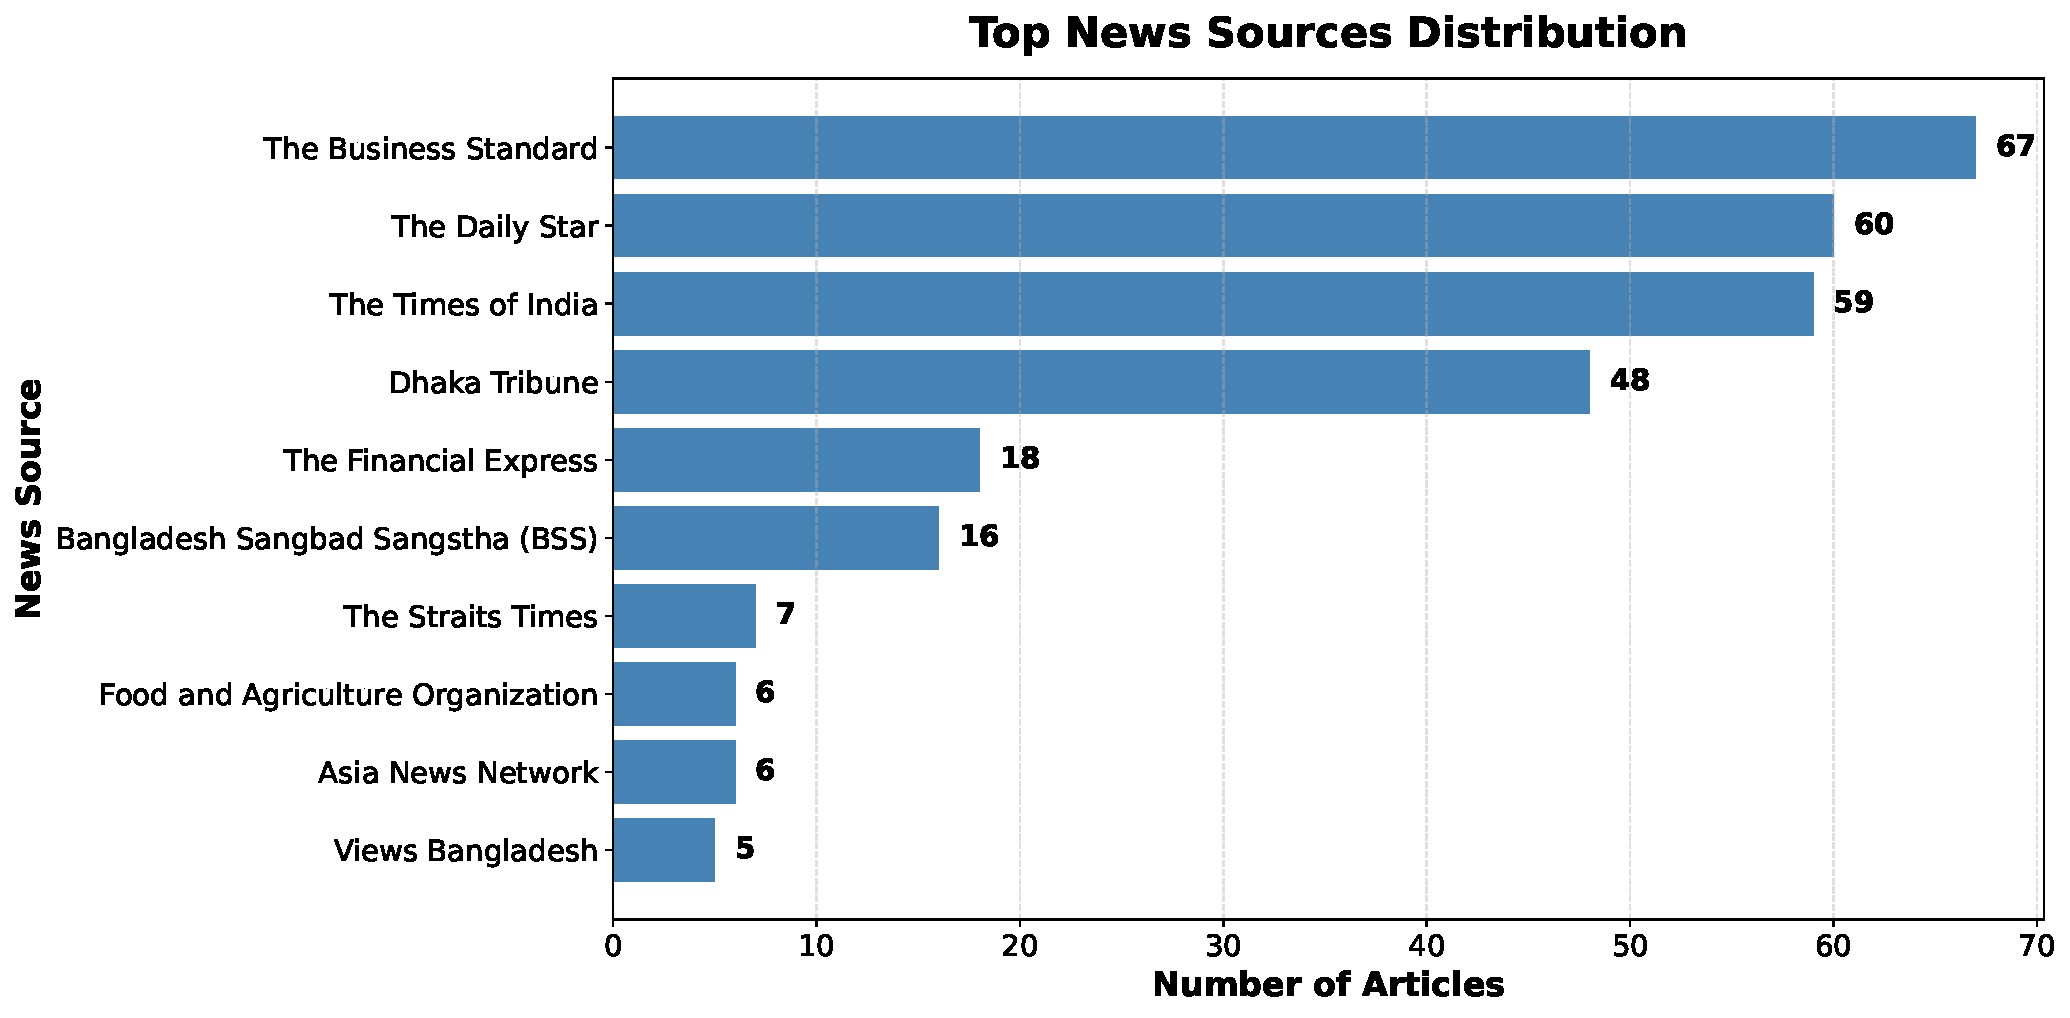
\includegraphics[width=0.90\linewidth]{figures/source_distribution.pdf}
\caption{Top News Sources Distribution}
\label{fig:source}
\end{figure}


\section{Discussion}

The results demonstrate that online news platforms can serve as a valuable source of information for studying stray animal abuse incidents and human-animal conflicts in Bangladesh. The collected data show that such incidents are reported across a wide range of news outlets, and the proposed framework is capable of converting these dispersed reports into a structured format suitable for analysis and decision-support purposes.

The findings further indicate that dog-related incidents constitute the largest portion of the dataset, whereas cat-related incidents and records with unidentified animal types occur less frequently. The existence of a substantial number of High-risk cases highlights the need for greater attention toward severe incidents such as poisoning, killing, abuse, and conflict-related events. These findings may assist animal welfare organizations, local authorities, and community stakeholders in prioritizing intervention efforts.

Several challenges were encountered during the implementation of the framework. First, many news headlines provide only limited information, which occasionally results in records being categorized as Unknown or Other. Second, location details are not consistently available within article metadata or headlines, restricting detailed geographical analysis in the current version of the system. Third, the framework currently relies on rule-based keyword classification, which offers transparency and simplicity but may not fully capture complex linguistic patterns or contextual meanings.

Despite these limitations, the proposed framework establishes a useful foundation for automated monitoring and analytical decision-support related to stray animal welfare. With additional data sources and more advanced analytical techniques, the system can be further enhanced to support researchers, NGOs, policymakers, and local authorities in identifying risk trends, monitoring incident patterns, and designing effective preventive strategies.

\section{Conclusion}

This research presented a data-driven analytical framework for monitoring and analyzing stray animal abuse incidents and human-animal conflicts in Bangladesh using information collected from online news sources. The proposed system performed automated data collection, preprocessing, incident classification, SARI-based risk assessment, and visualization to transform unstructured reports into structured analytical information.

The findings indicate that online news data can be utilized as a practical source for generating incident intelligence related to animal welfare and community safety. The proposed Stray Abuse Risk Index (SARI) offers a straightforward yet effective approach for assessing incident severity and identifying cases that may require greater attention or intervention.

Several opportunities exist for future enhancement of the framework. Potential improvements include expanding the dataset, incorporating full-text article analysis, applying advanced natural language processing techniques, improving geographical information extraction, generating district-level risk maps, and integrating information from social media platforms and NGO reports. Such extensions can improve the accuracy, scalability, and real-world applicability of the system while strengthening its role as a decision-support tool for animal welfare management and preventive intervention planning.

\bibliographystyle{IEEEtran}
\bibliography{references}

\end{document}

